% !TeX root = ../main.tex

Data can often be viewed as a sample of a function on some unknown space.
Determining if this sample sufficiently \emph{covers} the underlying space is a fundamental question for any meaningful analysis.
Taking the sample as points in some unknown metric space, coverage requires that the underlying space is contained in the union of metric balls centered at points in the sample.
The radius of these metric balls determines the scale at which the space is covered.
Often, data is provided without coordinates, and only pairwise connectivity information that indicates when sample points are within some fixed distance.
Testing for coverage in this setting is a problem that is essentially topological in nature.
Homology is a tool from algebraic topology that can be used to compute coverage holes from pairwise connectivity information alone.
% That is, given only pairwise connectivity information, homology can detect the holes in a cover that may indicate a lapse in coverage.
However, holes in a cover may not indicate a lack of coverage, as these holes may be properties of the underlying space.
Moreover, not all lapses in coverage appear as holes in the cover, as there may be regions of the space that have not bee sampled at all.
Verifying coverage therefore requires information about the boundary of the space that is captured by its homology.

The Topological Coverage Criterion (TCC) is a computable condition for coverage that uses homology along with topological priors in a coordinate-free setting.
That is, given only pairwise connectivity information, the TCC uses information about the boundary of a space to confirm coverage using relative homology.
In its original form this required that the sample points near the boundary were labelled manually---without coordinates, there is no way to determine these points analytically.
This requirement is perhaps the main reason why the TCC can so rarely be applied in practice.
For points sampled from a real-valued function, it can be shown that this requirement can be replaced with assumptions about the function itself.
One can then use prior information about the homology of the function above (or below) a given scalar value to confirm coverage of a \emph{part} of the domain.

While data coverage is an important property throughout data analysis, it has an important role to play in topological approaches to data.
These techniques provide novel information about the structure of data, and coverage provides a way to attribute that structure to the underlying space.
In particular, \emph{persistent homology} decomposes the homology of a space by a sequence of subspaces to produce a robust topological signature known as a persistence \emph{barcode} or \emph{diagram}.
For a real-valued function this sequence is defined by its sub or super level sets.
The resulting signature is invariant to continuous transformations, and is therefore a useful signature for use with non-deterministic statistical techniques in particular.
Topological Scalar Field Analysis (SFA) approximates the persistent homology of a real-valued function from a finite sample.
The fundamental assumption made in SFA is that this sample covers the domain at some scale, and the quality of the approximation is proportional to this scale.

\begin{figure}[htbp]
  \begin{minipage}{0.35\textwidth}
    \centering
    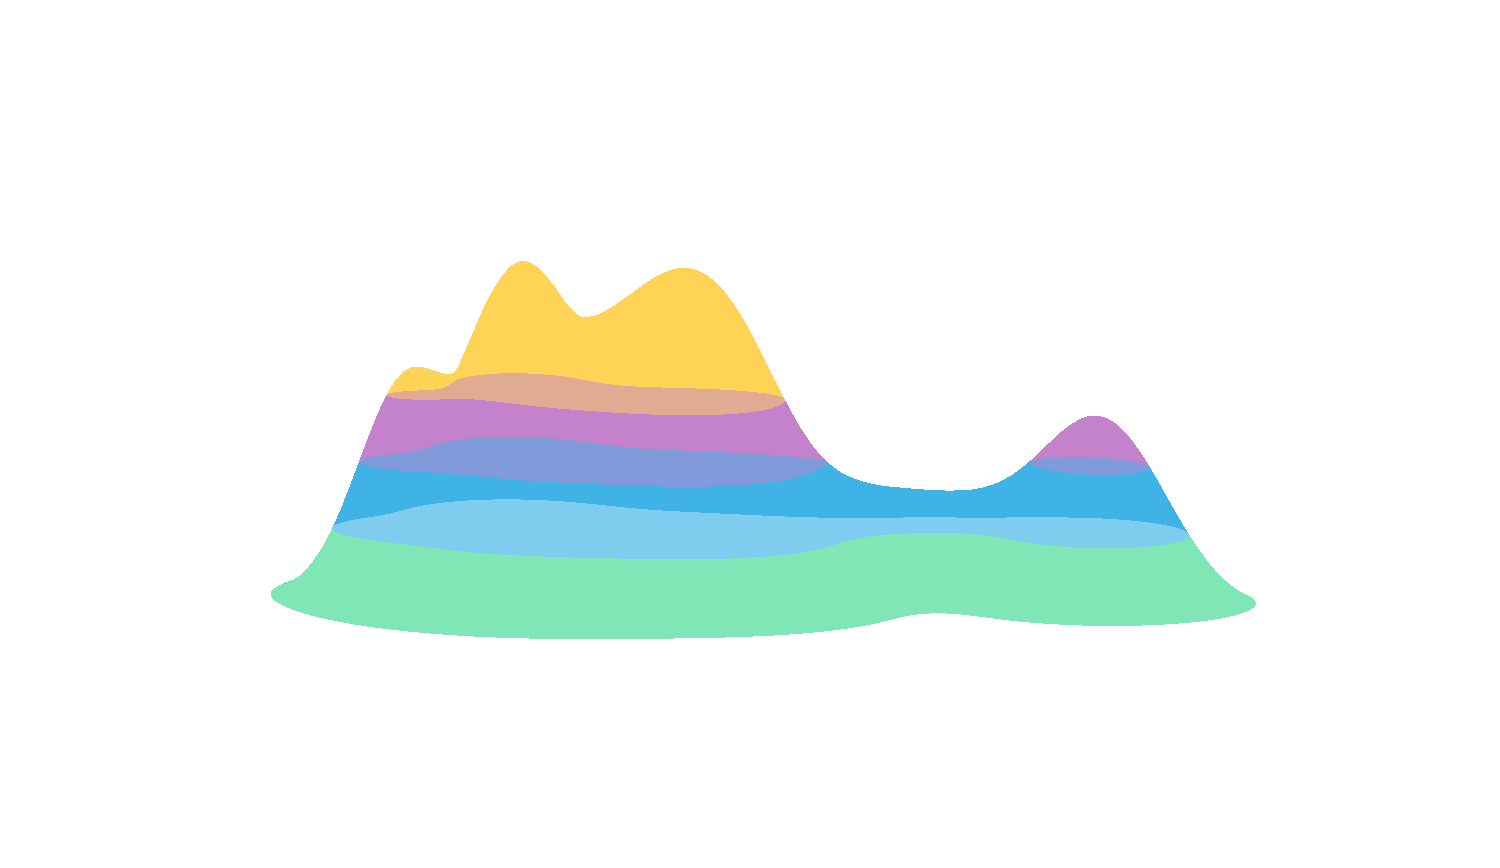
\includegraphics[trim=200 200 200 200, clip, width=0.8\linewidth]{figures/surf-side.png}
    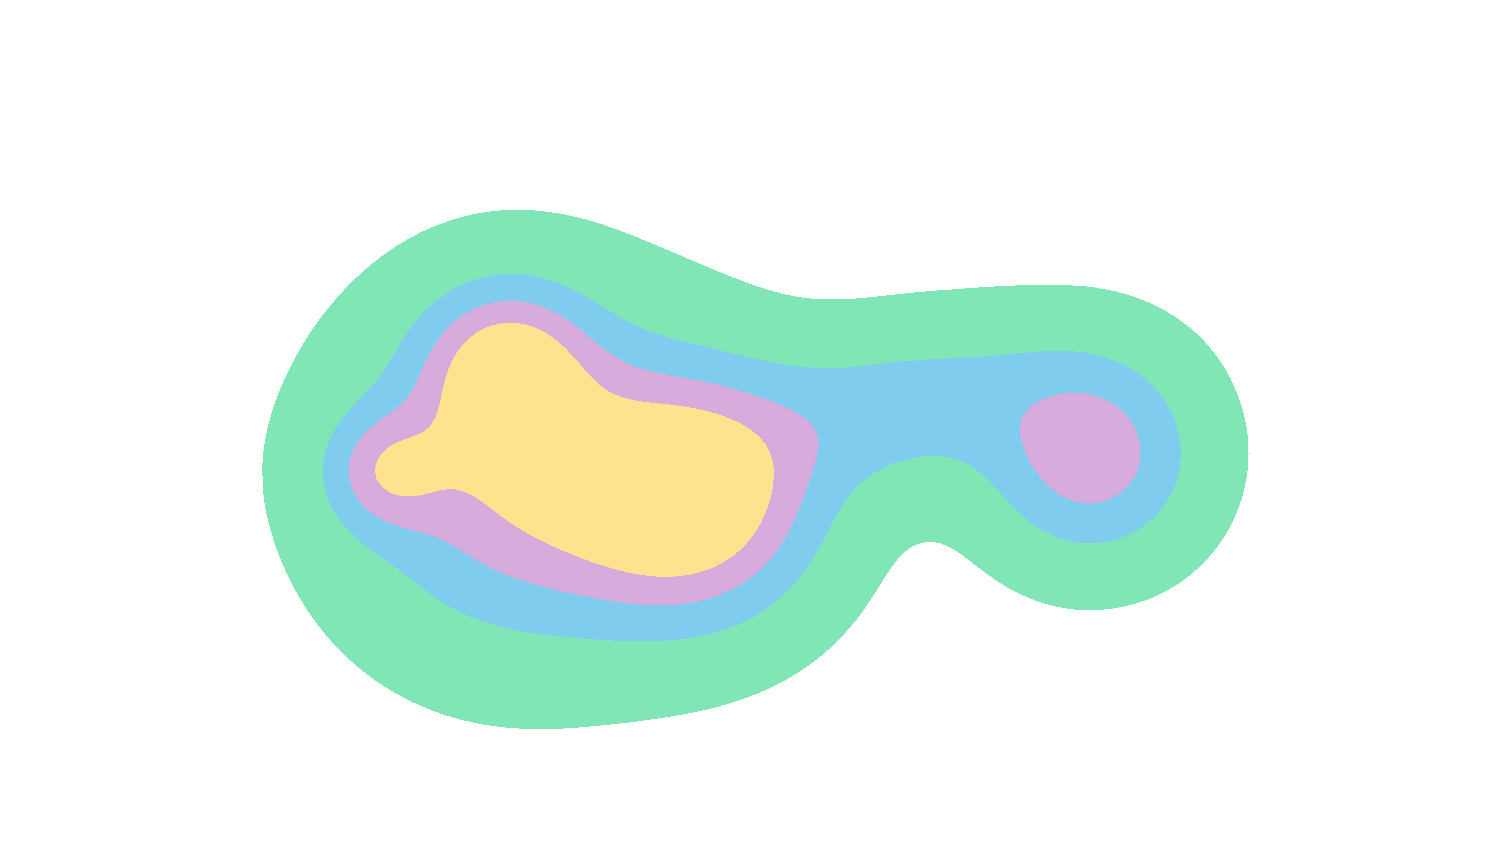
\includegraphics[trim=200 100 200 150, clip, width=0.75\linewidth]{figures/surf-top.png}
  \end{minipage}
  \begin{minipage}{0.5\textwidth}
    \centering
    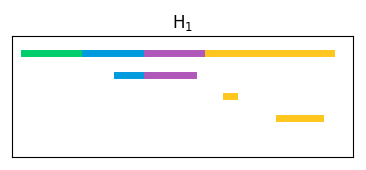
\includegraphics[width=\linewidth]{figures/scalar_barcode_H1.png}
  \end{minipage}
  \caption{A scalar field on a 2D domain and its persistent homology in dimension 1.}
\end{figure}

Given a finite sample of a real-valued function both the TCC and SFA apply homology in a coordinate-free setting.
By modifying the statement of the TCC information about the persistent homology of the function can be used as topological priors.
In fact, it can be shown that the TCC can be extracted from the persistent relative homology of a sample.
One can then verify the quality of an approximation directly from a variation of the signature computed in SFA.

\paragraph{Objectives}

% Moreover, this variation supports instances of partial coverage
The proposed work will unify the TCC and SFA as a way to provide verified scalar field analysis.
This first requires adapting the TCC to bounding subsets of the domain defined by the function itself.
It also requires a new stability proof for approximating the persistent homology of a real-valued function modulo a static.
In addition to providing a theoretical framework for the unification of these two theories, this work will explore the significance of the resulting relative persistent homology.

A key observation in this work is that the TCC confirms not only coverage, but that the sample is \emph{topologically representative} of the domain for a given range of function values.
Using this observation, a number of connections with existing work on Extended persistence and level set persistence will be explored.
In particular, the TCC can be viewed as confirming the presence of a \emph{fundamental class} that can be used to compute \emph{topological duals}.
Additional work is motivated by an application involving Lipschitz extensions that requires computing these topological duals within the persistence computation.
This will extend the existing theory of persistent (co)homology to support duality via the cap product with a fundamental class.

% Specifically, the objectives of this work are as follows:
%
% \begin{itemize}
%   \item A theorem for verified SFA that unifies the assumptions made by the TCC and those required by SFA.
%   \item An efficient algorithm for merging the relative persistence diagrams produced.
%   \item An investigation of how SFA can be used
% \end{itemize}
%
% the persistence diagram of the function
% One of the main goals is to provide a theorem for verified SFA that unifies the assumptions made by the TCC and those required by SFA
